% !TeX root = ../main.tex

\chapter{基于角色涌现的多智能体强化学习}
本章详细描述具体的基于角色的框架,以及考虑到“角色”应该具有的诸多性质,来设计损失函数,以引导“角色”涌现的完成。本章的结构为,首先介绍角色是什么,然后角色应该具有的四种性质,再然后引入让每个智能体的效用函数都基于自己的角色的方法,进一步再根据角色的性质设计用于优化的损失函数,最后再对总的损失函数进行总结。同时,为了让本框架更加容易理解,本章在后面还附加上另一种从深度学习角度的原理阐述。

\section{角色的定义}
为了不引起混淆,简要描述一下本文使用的角色的定义。

本文的角色是对某一行为模式的抽象。它应该具有如下的表现特征:

i) \textbf{具有某一角色的智能体常常专注于某一个或某一些子任务;}

ii) \textbf{具有相似角色的智能体会有相似的行为;}

拿蚂蚁来举例,一个蚂蚁群通常分为如下的角色:工蚁、兵蚁、蚁后等,具有工蚁角色的蚂蚁通常的行为是采集食物、建造巢穴、哺育幼蚁等,如果两只蚂蚁具有相似的角色(比如都是工蚁),那么它们的行为就会相似,具体来说,在蚂蚁这个案例里,这两只蚂蚁的每日的轨迹可能是重叠的。但是反过来,不同的角色,比如工蚁和兵蚁,它们的行为轨迹就会大不相同。

最后,角色本身是复杂的概念,很难做一个完整的定义,本文只关注那些比较明显的特征。


\section{角色具有的性质}
本小节介绍本项目认为的角色应该具有的性质。

从社会学的角度来说,角色应该会拥有很复杂、广泛的性质,比如某个角色可能会在与其他角色的交互中不断演化、越来越复杂。但是完全表达这些复杂的性质是没有必要的,本项目的目的是为了利用角色这一概念中对多智能体强化学习有启发的部分,因此,考虑到有效性和可行性,角色应该要具有如下的性质:

i) \textbf{可识别性(Identifiable)}: 一个智能体的角色能够通过它的行为模式识别出来。这一性质意味着,一个角色应该是与行为模式挂钩的,这一点正符合对角色的定义,即“角色是对某一行为模式的抽象”。

ii) \textbf{专业化(Specialized)}: 具有相似角色的智能体应该专门处理相似的子任务。这一性质同时也意味着处理相似的子任务的智能体应该也是相似的角色。

iii) \textbf{动态(Dynamic)}: 一个智能体的角色应该能动态地变化,并且这种变化是为了适应环境。正如上文所说,角色会随着和环境、其他角色的交互不断演化。

iv) \textbf{通用性(Versatile)}: 涌现出来的角色应该足够不同,这样才能处理那些需要不同角色的任务。比如蚁群的生存繁衍任务,就需要工蚁、兵蚁、蚁后等角色才能完成。


\section{基于角色的智能体}
在表达上一节的性质之前,需要先设计如何让一个智能体基于角色来决策。

注意到,在现在的多智能体系统中,每个智能体$i$都有一个局部的效用函数(或者一个局部的策略函数),为了让智能体是基于自己的角色的,让该智能体的局部效用(策略)函数的参数$\theta_i$决定于它自己的角色$\rho_i$. 

同时,为了让学到的角色拥有上面表述的性质,将角色编码到随机嵌入空间(stochastic embedding space), 在这个基础上,让每个智能体$i$的角色$\rho_i$采样自一个多维高斯分布,即$\mathcal{N}(\bm{\mu}_{\rho_i}, \bm{\sigma}_{\rho_i})$.

\section{框架结构图}
为了便于后续的长文的理解,这里提前给出完整的框架图。

\begin{figure*}
    \centering
    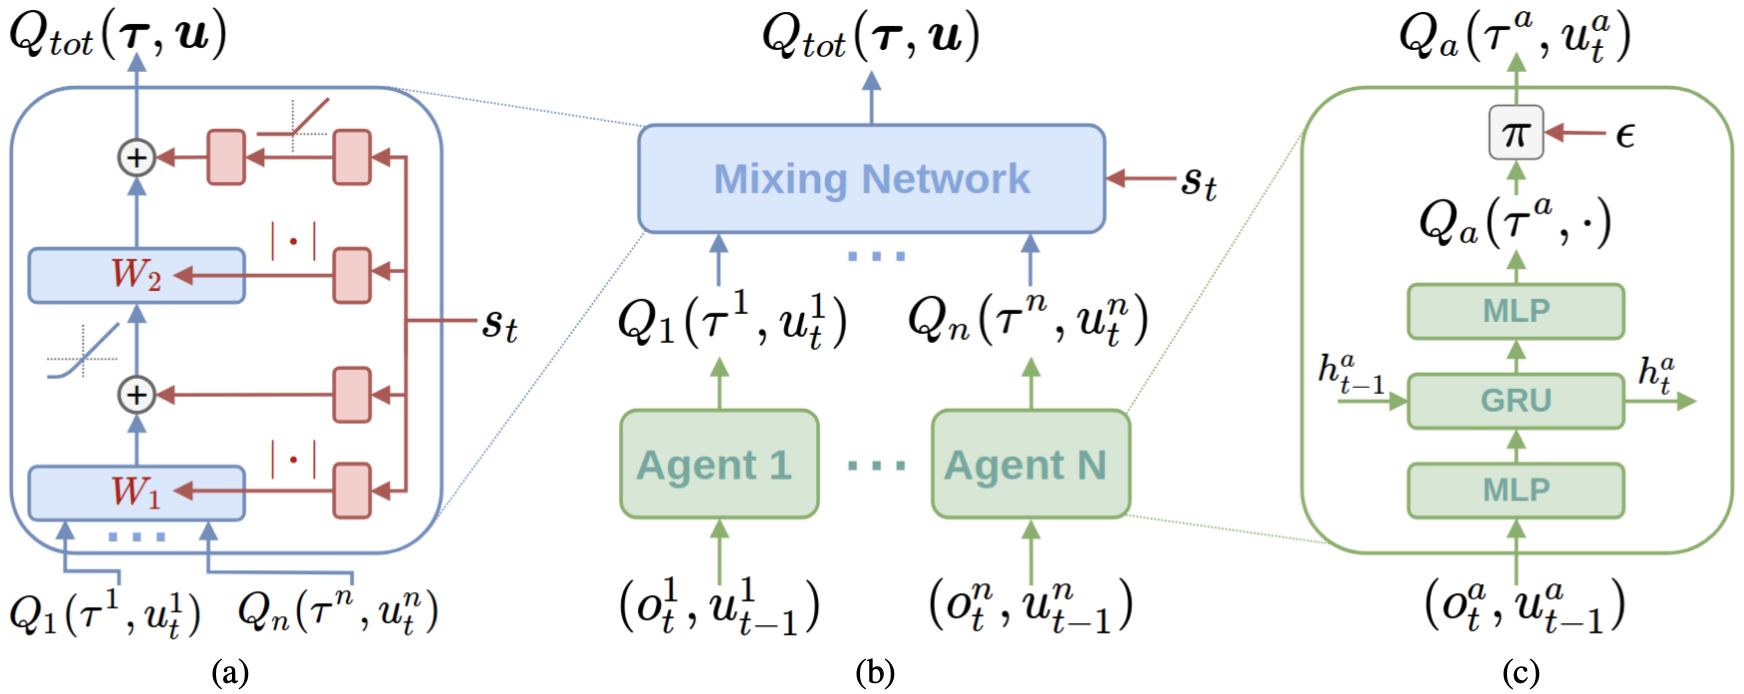
\includegraphics[width=0.8\linewidth]{figures/framework/qmix_framework.png}
    \caption{QMIX的框架图}
    \label{fig:qmix_framework}
    \note{(a)是混合网络的结构(蓝色), 它的权重和偏置是又一个超网络(hyper-net)(红色)得到的。 (b)是QMIX的整体框架结构图。(c)是局部效用函数图。}
\end{figure*}

前文叙述到,可以将智能体的局部效用函数或者局部策略函数决定于该智能体的角色,本项目在实践上使用的是局部效用函数,并且采用QMIX~\cite{rashid2018qmix}的基本框架,它的框架图为图~\ref{fig:qmix_framework}.

\begin{figure}
    \centering
    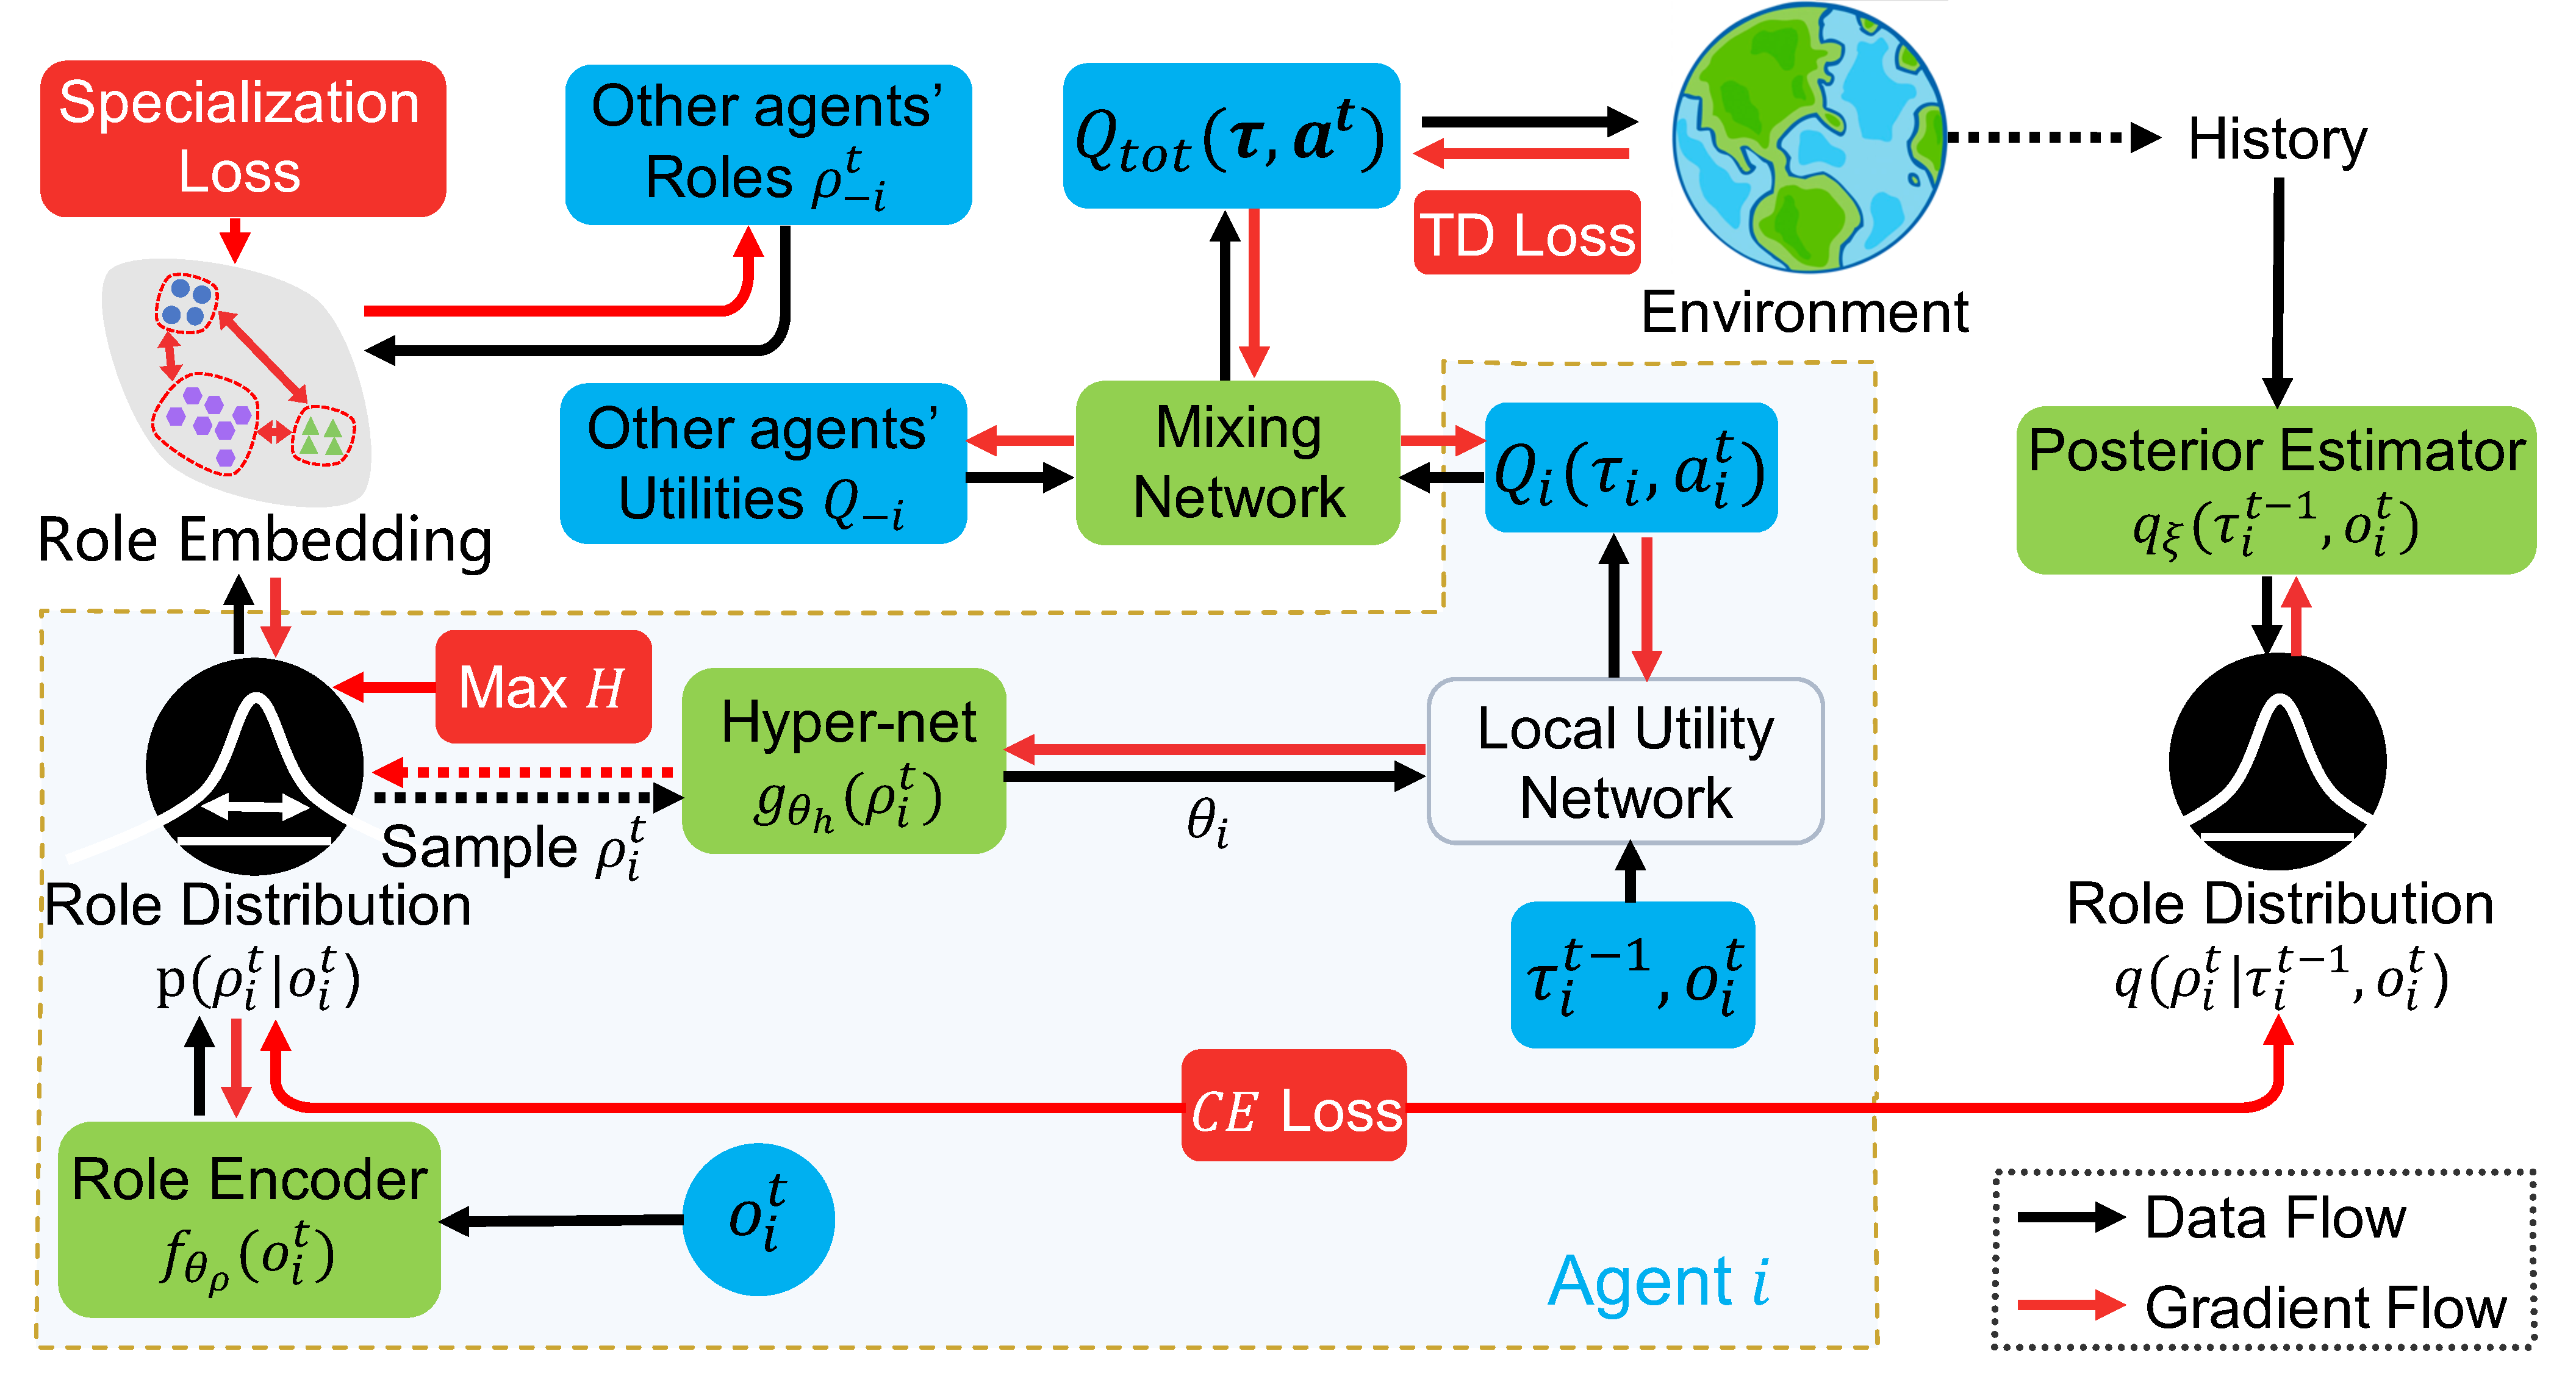
\includegraphics[width=0.95\linewidth]{figures/framework/framework.pdf}
    \caption{本项目的框架图}
    \label{fig:framework}
    \note{角色编码器产生一个在角色嵌入空间的多维高斯分布,从这个分布里采样得到一个角色,然后作为输入给一个超网络,输出得到局部效用函数的参数,即权重和偏置。局部效用函数得到的值再集中进入到一个混合网络,得到整体动作的值的一个估计。在智能体和环境以及其他智能体的交互中,个体的轨迹被收集起来,然后进入到轨迹编码器,得到角色分布的后验估计。整个框架使用端到端的方式训练。}
\end{figure}

本项目的框架图为图~\ref{fig:framework}

\section{角色的性质及损失函数设计}
前面介绍了如何将智能体基于自己的角色来决策,并且给出了基本角色应该具有的四个性质,下面将结合基本框架,设计损失函数,使得最终学到的角色满足上面的性质。

\subsection{角色的动态变化性质}
角色的动态变化性质是指,一个智能体的角色能够为了适应环而动态地变化。为了班组这个性质,将智能体的角色取决于它自己的局部观测,上文提到角色是采样自一个多维高斯分布,在此基础上,使用一个输入为智能体局部观测的可训练的神经网络$f$来学习这个多维高斯分布的参数,即$\bm{\mu}_{\rho_i}$和$\bm{\sigma}_{\rho_i}$, 完整的表达如下:
\begin{equation}
\begin{aligned}
(\bm{\mu}_{\rho_i}, \bm{\sigma}_{\rho_i}) &= f(o_i; \theta_\rho), \\
\rho_i &\sim \mathcal{N}(\bm{\mu}_{\rho_i}, \bm{\sigma}_{\rho_i}),
\end{aligned}
\end{equation}
其中,$\theta_\rho$ 是神经网络$f$的参数,$o_i$是智能体的局部观测。

得到多维高斯分布之后采样得到角色$\rho_i$, 然后该角色经过一个超网络(hyper-network)$g(\rho_i;\theta_h)$(其中$\theta_h$为该超网络的参数)处理得到局部效用函数的参数$\theta_i$. 在下文中,将会把$f$称为角色编码器(role encoder), 把$g$称为角色解码器(role decoder),这一点类似自动编码器(auto-encoder)结构。

\subsection{角色的可识别性和通用性}
注意到,上述引入角色的随机嵌入空间和将角色决定于每个智能体自己的局部观测,并不能得到一个满足通用性和可识别性的角色,因为目前没有引入别的信息来满足这一点。

\subsubsection{条件互信息建模}
为了满足通用性,即让角色在决定于局部观测$o_i$的条件下足够地不同,可以最大化一个信息熵$H(\rho_i|o_i)$. 另一方面,为了满足可识别性,可以在给定路径$\tau_i$信息条件下最小化条件熵$H(\rho_i | \tau_i, o_i)$.

结合这两个熵,只需要去最大化$H(\rho_i | o_i) - H(\rho_i | \tau_i, o_i)$, 在数学上,这个式子等价于$I(\tau_i; \rho_i | o_i)$, 也就是关于每个智能体自己的路径$\tau_i$和基于当前观测$o_i$的角色$\rho_i$之间的的条件互信息。

\subsubsection{条件互信息的下界}
然而,直接去估计和最大化互信息往往是不可行的,因为它们的数值无法直接得到。为了解决这个问题,采用变分推断~\cite{wainwright2008graphical, alemi2017deep}.

引入一个变分后验估计来得到一个可以处理的关于互信息的下界,注意到这里是针对每个时刻$t$:
\begin{align*}
    I(\rho^t_i; \tau^{t-1}_i | o^t_i) & = \mathbb{E}_{\rho^t_i, \tau^{t-1}_i, o^t_i}\left[\log\frac{p(\rho^t_i | \tau^{t-1}_i, o^t_i)}{p(\rho^t_i | o^t_i)}\right] \\
    & = \mathbb{E}_{\rho^t_i, \tau^{t-1}_i, o^t_i}\left[\log\frac{q_\xi(\rho^t_i | \tau^{t-1}_i, o^t_i)}{p(\rho^t_i | o^t_i)}\right] \\ & \ \ \ \ + \mathbb{E}_{\tau^{t-1}_i, o^t_i}\left[\KL(p(\rho^t_i|\tau^{t-1}_i, o^t_i) \| q_\xi(\rho^t_i|\tau^{t-1}_i, o^t_i))\right] \\
    & \ge  \mathbb{E}_{\rho^t_i, \tau^{t-1}_i, o^t_i}\left[\log\frac{q_\xi(\rho^t_i | \tau^{t-1}_i, o^t_i)}{p(\rho^t_i | o^t_i)}\right]\stepcounter{equation}\tag{\theequation}
    \label{equ:mi}
 \end{align*}
其中,轨迹$\tau^{t-1}_i=(o_i^0, a_i^0, \cdots, o_i^{t-1}, a_i^{t-1})$, $q_\xi$是一个变分估计,它的参数是$\xi$. 另外最后一个不等式成立是因为KL散度的非负性。

分布$q_\xi$可以是任意的,这里使用一个GRU~\cite{cho2014learning}来编码每个智能体自己的历史观测和动作,这个结构称之为轨迹编码器(trajectory encoder).

为了便于最小化,公式~\ref{equ:mi}中的下界可以进一步表达成一个损失函数的形式:
\begin{align*}
    \mathcal{L}_I(\theta_\rho, \xi) = & \mathbb{E}_{(\tau^{t-1}_i, o^t_i)\sim D}\big[\mathcal{CE}[p(\rho^{t}_i | o^t_i)\| q_\xi(\rho^{t}_i | \tau^{t-1}_i, o^t_i)] - H(\rho^{t}_i | o^t_i)\big],\stepcounter{equation}\tag{\theequation}
\end{align*}
其中,$\mathcal{D}$是缓存,$H(\cdot)$是熵,$\mathcal{CE[\cdot\|\cdot]}$是交叉熵。推导如下。

\subsubsection{损失函数的推导}
上面得到关于条件互信息的如下下界:
\begin{equation}
    I(\rho^t_i; \tau^{t-1}_i | o^t_i) \ge  \mathbb{E}_{\rho^t_i, \tau^{t-1}_i, o^t_i}\left[\log\frac{q_\xi(\rho^t_i | \tau^{t-1}_i, o^t_i)}{p(\rho^t_i | o^t_i)}\right]
    \label{equ:mi-2}
 \end{equation}
进一步可以得到:
\begin{equation}
    \begin{aligned}
       &\mathbb{E}_{\rho^t_i, \tau^{t-1}_i, o^t_i}\left[\log\frac{q_\xi(\rho^t_i | \tau^{t-1}_i, o^t_i)}{p(\rho^t_i | o^t_i)}\right]\\
      =&\mathbb{E}_{\rho^t_i, \tau^{t-1}_i, o^t_i}\left[\log q_\xi(\rho^t_i | \tau^{t-1}_i, o^t_i)\right]-\mathbb{E}_{\rho^t_i, o^t_i}\left[\log p(\rho^t_i | o^t_i)\right]\\
      =&\mathbb{E}_{\rho^t_i, \tau^{t-1}_i, o^t_i}\left[\log q_\xi(\rho^t_i | \tau^{t-1}_i, o^t_i)\right]+\mathbb{E}_{o^t_i}\left[H(\rho_i^t | o_i^t)\right] \\
      =&\mathbb{E}_{\tau^{t-1}_i, o^t_i}\left[\int p(\rho^t_i | \tau^{t-1}_i, o^t_i) \log q_\xi(\rho^t_i | \tau^{t-1}_i, o^t_i)d\rho^t_i\right] +\mathbb{E}_{o^t_i}\left[H(\rho_i^t | o_i^t)\right]
       \label{equ:mi_derivation}
    \end{aligned}
\end{equation}
注意到,角色编码器(role encoder)决定于局部观测,所以给定局部观测,角色的分布$p(\rho^t_i)$与局部历史轨迹$\tau^{t-1}_i$独立。从而得到:
\begin{equation}
    \begin{aligned}
          I(\rho^t_i; \tau^{t-1}_i | o^t_i) 
      \ge -\mathbb{E}_{\tau^{t-1}_i, o^t_i}\left[\mathcal{CE}[p(\rho^t_i | o^t_i) \| q_\xi(\rho^t_i | \tau^{t-1}_i, o^t_i)\right] +    \mathbb{E}_{o^t_i}\left[H(\rho_i^t | o_i^t)\right]
       \label{equ:mi_assumption}
    \end{aligned}
\end{equation}
在实验上,会使用一个缓存$\mathcal{D}$来采样得到轨迹数据,然后最小化如下的损失函数:
\begin{equation}
    \begin{aligned}
        \mathcal{L}_I(\theta_\rho, \xi) = \mathbb{E}_{(\tau^{t-1}_i, o^t_i)\sim\mathcal{D}}\left[\mathcal{CE}[p(\rho^t_i | o^t_i) \| q_\xi(\rho^t_i | \tau^{t-1}_i, o^t_i) - H(\rho_i^t | o_i^t)\right].
    \end{aligned}
\end{equation}

\subsection{角色的专业化性质}
到目前为止,并没有一个推动子任务专业化的引导,而这一点是分解一整个任务和提高多智能体性能的关键。具体来说,上述的最小化损失函数$\mathcal{L}_I$能够让角色含有足够的包含长期历史行为的信息,但是这个并没有显式地确保有相似行为的智能体有相近的角色,特别地,本文指在随机嵌入空间里的角色。

从直觉上来说,在一个集体中,对于任意两个有明确子任务的智能体,要么它们有相似的角色,从事相似的任务,要么它们角色完全不一样,行为轨迹完全不同。但是,在角色涌现的过程中,智能体是否拥有相似的角色是不知道的,同时,行为轨迹的相似性也不容易直接定义。

为了解决这个问题,引入一个新的规范项。

\subsubsection{不相似性矩阵的引入}
让两个智能体$i$和$j$有相似的角色和相似的行为,可以最大化关于智能体$i$角色和智能体$j$行为的互信息$I(\rho_i; \tau_j)$. 但是,直接优化这个最大化项会导致所有的智能体有相同的角色,这是和设计违背的,并且会拉低性能。为了解决这个问题,引入一个不相似性模型$d_{\phi}: \Tau\times\Tau\rightarrow\mathbb{R}$, 这是一个已两个轨迹作为输入的可训练的神经网络。然后去最大化$I(\rho_i; \tau_j) + d_\phi(\tau_i, \tau_j)$, 与此同时,最小化矩阵$D_\phi=(d_{ij})$中非零元素的个数,其中$d_{ij}=d_\phi(\tau_i, \tau_j)$是估计的两个智能体$i$和$j$的轨迹的不相似性。

这样的优化方式能够保证,不相似性$d$只有当互信息$I$很低时很高,这样的结果就是学到的角色在随机嵌入空间或者角色空间很紧密但是又有足够的多样化来分别解决不同的子任务。

\subsubsection{不相似性优化的数学表达}
从数学上,上述的优化方式可以写成如下形式:
\begin{align*}
    &\underset{{\theta_\rho, \xi, \phi}}{\text{minimize}} \ \ \ \|D_\phi^t\|_{2,0} \stepcounter{equation}\tag{\theequation} \\
    &\text{subject to} \ \ \ I(\rho^{t}_i; \tau^{t-1}_j|o^t_j) + d_\phi(\tau^{t-1}_i, \tau^{t-1}_j) > U, \forall i\ne j
\end{align*}
其中,$U$是用来控制角色表征的紧密程度的超参。

使用Frobenius来放松上面的优化形式,可以得到如下的最小化优化项:
\begin{equation}
\begin{aligned}
    \|D_\phi^t\|_{F} - \sum_{i\ne j}\min\{I(\rho^{t}_i; \tau^{t-1}_j|o^t_j) + d_\phi(\tau^{t-1}_i, \tau^{t-1}_j), U\},
\end{aligned}
\end{equation}

和上一节一样,直接估计和优化互信息是不能处理的,这里还是采用变分后验推断来得到一个上界:
\begin{align*}
    \mathcal{L}_D(\theta_\rho, \phi, \xi) = &\mathbb{E}_{(\bm{\tau}^{t-1}, \bm{o}^t)\sim\mathcal{D}, \bm{\rho}^t\sim p(\bm{\rho}^t | \bm{o}^t)}\big[\|D_\phi^t\|_{F} \stepcounter{equation}\tag{\theequation} \\ 
        & - \sum_{i\ne j}\min\{q_\xi(\rho^{t}_i| \tau^{t-1}_j, o^t_j) + d_\phi(\tau^{t-1}_i, \tau^{t-1}_j), U\}\big]
\end{align*}
其中,$\mathcal{D}$是缓存,$\bm{\tau}^{t-1}$是联合的轨迹,$\bm{o}^{t}$是联合的观测,以及$\bm{\rho}^{t}=\langle \rho_1^t, \rho_2^t, \cdots, \rho_n^t\rangle$. 具体推导如下:

\subsubsection{损失函数的推导}
首先,
\begin{equation}
    \begin{aligned}
    I(\rho^{t}_i; \tau^{t-1}_j | o^t_j) &= \mathbb{E}_{\rho^{t}_i, \tau^{t-1}_j, o^t_j}\left[\log\frac{p(\rho^{t}_i, \tau^{t-1}_j | o^t_j)}{p(\rho^{t}_i | o^t_j)p(\tau^{t-1}_j | o^t_j)}\right] \\
    &= \mathbb{E}_{\rho^{t}_i, \tau^{t-1}_j, o^t_j}\left[\log\frac{p(\rho^{t}_i| \tau^{t-1}_j, o^t_j)}{p(\rho^{t}_i | o^t_j)}\right] \\
    &= \mathbb{E}_{\rho^{t}_i, \tau^{t-1}_j, o^t_j}\left[\log p(\rho^{t}_i| \tau^{t-1}_j, o^t_j)\right] + \mathbb{E}_{o^t_j}\left[H(\rho^{t}_i | o^t_j)\right]\\
    &\ge \mathbb{E}_{\rho^{t}_i, \tau^{t-1}_j, o^t_j}\left[\log p(\rho^{t}_i| \tau^{t-1}_j, o^t_j)\right].
    \end{aligned}
\end{equation}
最后一个不等式成立的原因是,实践上将角色分布(即一个多维高斯分布)的方差的下界固定到一个值,使得分布的熵总是非负的。

然后可以推出下面:
\begin{equation}
    \begin{aligned}
    &\mathbb{E}_{\rho^{t}_i, \tau^{t-1}_j, o^t_j}\left[\log p(\rho^{t}_i| \tau^{t-1}_j, o^t_j)\right] \\
    =& \mathbb{E}_{\rho^{t}_i, \tau^{t-1}_j, o^t_j}\left[\log q_\xi(\rho^{t}_i| \tau^{t-1}_j, o^t_j)\right] + \mathbb{E}_{\tau^{t-1}_j, o^t_j}\left[\KL\left[p(\rho^{t}_i| \tau^{t-1}_j, o^t_j) \| q_\xi(\rho^{t}_i| \tau^{t-1}_j, o^t_j) \right]\right] \\
    \ge & \mathbb{E}_{\rho^{t}_i, \tau^{t-1}_j, o^t_j}\left[\log q_\xi(\rho^{t}_i| \tau^{t-1}_j, o^t_j)\right]\label{equ:s_lower_bound},
    \end{aligned}
\end{equation}
其中,$q_\xi$是轨迹编码器。最后一个不等式成立是因为KL散度的非负性。

从而得到:
\begin{equation}
    \begin{aligned}
    I(\rho^{t}_i&; \tau^{t-1}_j | o^t_j) \ge \mathbb{E}_{\rho^{t}_i, \tau^{t-1}_j, o^t_j}\left[\log q_\xi(\rho^{t}_i| \tau^{t-1}_j, o^t_j)\right].\label{equ:t1get2}
    \end{aligned}
\end{equation}

上文中,提出关于角色的专业化性质可以最小化:
\begin{equation}
    \begin{aligned}
    \|D_\phi^t\|_{F} - \sum_{i\ne j}\min\{I(\rho^{t}_i; \tau^{t-1}_j|o^t_j) + d_\phi(\tau^{t-1}_i, \tau^{t-1}_j), U\},\label{equ:raw_obj}
    \end{aligned}
\end{equation}

对于这一项$\min\{I(\rho^{t}_i; \tau^{t-1}_j|o^t_j) + d_\phi(\tau^{t-1}_i, \tau^{t-1}_j), U\}$, 可以得到:
\begin{equation}
    \begin{aligned}
    &\min\{I(\rho^{t}_i; \tau^{t-1}_j|o^t_j) + d_\phi(\tau^{t-1}_i, \tau^{t-1}_j), U\} \\ = &\min\{\mathbb{E}_{\bm{\tau}^{t-1}, \bm{o}^t, \bm{\rho}^t}\left[\log\frac{p(\rho^{t}_i, \tau^{t-1}_j | o^t_j)}{p(\rho^{t}_i | o^t_j)p(\tau^{t-1}_j | o^t_j)} + d_\phi(\tau^{t-1}_i, \tau^{t-1}_j)\right], \mathbb{E}_{\bm{\tau}^{t-1}, \bm{o}^t, \bm{\rho}^t}\left[U\right]\},
    \end{aligned}
\end{equation}

为了简化起见,定义符号,
\begin{equation}
    \begin{aligned}
    T_1 &\equiv \log\frac{p(\rho^{t}_i, \tau^{t-1}_j | o^t_j)}{p(\rho^{t}_i | o^t_j)p(\tau^{t-1}_j | o^t_j)},\\
    T_2 &\equiv \log q_\xi(\rho^{t}_i| \tau^{t-1}_j, o^t_j).
    \end{aligned}
\end{equation}

由于
\begin{equation}
    \begin{aligned}
    T_2 &\ge \min\{T_2, U\}, \\
    U &\ge \min\{T_2, U\},
    \end{aligned}
\end{equation}

可以得到:
\begin{equation}
    \begin{aligned}
    \mathbb{E}_{\bm{\tau}^{t-1}, \bm{o}^t, \bm{\rho}^t}\left[T_2\right] &\ge \mathbb{E}_{\bm{\tau}^{t-1}, \bm{o}^t, \bm{\rho}^t}\left[\min\{T_2, U\}\right], \\
    \mathbb{E}_{\bm{\tau}^{t-1}, \bm{o}^t, \bm{\rho}^t}\left[U\right] &\ge \mathbb{E}_{\bm{\tau}^{t-1}, \bm{o}^t, \bm{\rho}^t}\left[\min\{T_2, U\}\right].\label{equ:xygemin}
    \end{aligned}
\end{equation}

从而,
\begin{equation}
    \begin{aligned}
     &\min\{\mathbb{E}_{\bm{\tau}^{t-1}, \bm{o}^t, \bm{\rho}^t}\left[T_1\right], \mathbb{E}_{\bm{\tau}^{t-1}, \bm{o}^t, \bm{\rho}^t}\left[U\right]\} \\
     \ge &\min\{\mathbb{E}_{\bm{\tau}^{t-1}, \bm{o}^t, \bm{\rho}^t}\left[T_2\right], \mathbb{E}_{\bm{\tau}^{t-1}, \bm{o}^t, \bm{\rho}^t}\left[U\right]\} \ \ \ \ \{\text{Eq.~\ref{equ:t1get2}}\} \\
     \ge & \mathbb{E}_{\bm{\tau}^{t-1}, \bm{o}^t, \bm{\rho}^t}\left[\min\{T_2, U\}\right] \ \ \ \ \{\text{Eq.~\ref{equ:xygemin}}\}, \label{equ:minexpectation}
    \end{aligned}
\end{equation}

这意味着,公式~\ref{equ:raw_obj}满足
\begin{align*}
    &\|D_\phi^t\|_{F} - \sum_{i\ne j}\min\{I(\rho^{t}_i; \tau^{t-1}_j|o^t_j) + d_\phi(\tau^{t-1}_i, \tau^{t-1}_j), U\} \\
  = & \mathbb{E}_{\bm{\tau}^{t-1}, \bm{o}^t, \bm{\rho}^t}\left[\|D_\phi^t\|_{F}\right] - \sum_{i\ne j}\min \{ \mathbb{E}_{\bm{\tau}^{t-1}, \bm{o}^t, \bm{\rho}^t}\left[T_1+d_\phi(\tau^{t-1}_i, \tau^{t-1}_j)\right], U\}\\ \stepcounter{equation}\tag{\theequation}\label{equ:specialized_math_lower_bound}
  \le & \mathbb{E}_{\bm{\tau}^{t-1}, \bm{o}^t, \bm{\rho}^t}\left[\|D_\phi^t\|_{F}\right] - \sum_{i\ne j}\mathbb{E}_{\bm{\tau}^{t-1}, \bm{o}^t, \bm{\rho}^t}\left[\min \{ T_2+d_\phi(\tau^{t-1}_i, \tau^{t-1}_j), U\}\right] \ \ \ \ \{\text{Eq.~\ref{equ:minexpectation}}\}\\
  = & \mathbb{E}_{\bm{\tau}^{t-1}, \bm{o}^t, \bm{\rho}^t}\left[\|D_\phi^t\|_{F} - \sum_{i\ne j}\min \{ T_2+d_\phi(\tau^{t-1}_i, \tau^{t-1}_j), U\}\right].
\end{align*}

从而可以最大化这个上界来优化公式~\ref{equ:raw_obj}. 

在实践上,可以最小化如下的损失函数:
\begin{align*}
    \mathcal{L}_D(\theta_\rho, \phi, \xi) = &\mathbb{E}_{(\bm{\tau}^{t-1}, \bm{o}^t)\sim\mathcal{D}, \bm{\rho}^t\sim p(\bm{\rho}^t | \bm{o}^t)}\big[\|D_\phi^t\|_{F} \stepcounter{equation}\tag{\theequation} \\ 
        & - \sum_{i\ne j}\min\{q_\xi(\rho^{t}_i| \tau^{t-1}_j, o^t_j) + d_\phi(\tau^{t-1}_i, \tau^{t-1}_j), U\}\big]
\end{align*}
$\mathcal{D}$是缓存,$\bm{\tau}^{t-1}$是联合的轨迹,$\bm{o}^{t}$是联合的观测,以及$\bm{\rho}^{t}=\langle \rho_1^t, \rho_2^t, \cdots, \rho_n^t\rangle$.

\subsection{总损失函数}
到现在已经介绍了三个损失函数,除了这些损失函数带来的梯度,在这个框架下的参数也会被TD损失更新。正如图~\ref{fig:framework}描述的那样,为了计算全局的TD损失,每个智能体自己的效用值会和其他的集合起来进入到全局的动作-值函数$Q_{tot}$. 本项目采用的是QMIX~\cite{rashid2018qmix}的混合函数,其实也很容易换用其他的。这里混合函数的参数决定于全局的状态$s$, 然后是使用一个超网络得到的,这个超网络的参数为$\theta_m$. 总结来说,整个的目标函数为:
\begin{equation}
    \mathcal{L}(\theta) = \mathcal{L}_{TD}(\theta) +\lambda_I\mathcal{L}_I(\theta_\rho, \xi) + \lambda_D\mathcal{L}_D(\theta_\rho, \xi, \phi),
\end{equation}
其中,$\theta=(\theta_\rho, \xi, \phi, \theta_h, \theta_m)$, $\lambda_I$和$\lambda_D$是用来调节损失函数相对大小的超参,以及$\mathcal{L}_{TD}(\theta)$ = $[r + \gamma \max_{\va'} Q_{tot}(s', \bm{a'}; \theta^-)$-$Q_{tot}$($s, \bm{a}; \theta$)$]^2$ ($\theta^-$是按固定周期更新的目标网络Target Network).

由于采用集中训练,分离执行(centralized training with decentralized execution paradigm, CTDE), 在分离执行的时候,仅仅有角色编码器、角色解码器和局部效用函数在起作用。

\section{其他阐释方式}
为了便于理解本框架为什么有效,这里另外给出一种解释。

为了获得可拓展性,现在的多智能体深度强化学习框架往往采用一个很简化的模式,即所有的智能体都共享以及学习一个分离的值网络或者策略网路,但是这样简单的共享往往是不够的,特别是对于一些复杂的多智能体任务。举例来说,在Adam Smith的大头针工厂里,工人必须要完成18个完全不同的子任务才能制作成一个大头针~\cite{smith1937wealth}。在这个情形下,只用一个共享的网络往往是很重的负担,因为它要同时去学很多完全不同的策略,还要去表达不同的技能。

在另一方面,每个智能体都单独有一个网络也是没必要的,因为有一些工人会有相同的任务,并且各自独立也会增加计算复杂度。

所以本项目解决的就是拥有相似任务的智能体共享一个网络,同时也会共享训练数据,也就是有相似的角色;而拥有不同任务的智能体则是不同的网络。结合上文,这里的网络(即局部效用函数网络)的参数(即权重和偏置)是使用角色产生。自然而然的,相似角色产生的网络相似,它们也会共享训练数据,不同角色产生的网络不同,它们不会干扰彼此。

\section{本章小结}

本章首先介绍角色是什么,即角色是行为模式的抽象。然后介绍角色应该具有的四种性质,即动态性、可识别性、通用性和专业化。再然后引入让每个智能体的效用函数都基于自己的角色的方法,即使用一个基于角色的超网络来产生局部效用函数的参数。进一步再根据角色的性质设计用于优化的损失函数。最后再对总的损失函数进行总结。同时,为了让本框架更加容易理解,本章在后面还附加上另一种从深度学习角度的原理阐述。